\documentclass[11pt,a4paper]{article}

% package importing
%\usepackage[margin=2cm]{geometry}
\usepackage{geometry}
 \geometry{
 a4paper,
 %total={170mm,257mm},
 left=20mm,
 top=20mm,
 right=20mm,
 bottom=20mm,
 }
 		%$$$$$$ fonts settings $$$$$$%
%\usepackage[sc]{mathpazo}  %for palatino font
%\usepackage{eulervm}  %for Euler maths font

		%$$$$$$ package imports $$$$$$%
\usepackage{amsmath}  %for mathematics
\usepackage{titlesec}  %for title spacing only
\usepackage{lipsum}  %random huge text generation
\usepackage{titlesec} %for changing font of titles 
\usepackage{amssymb}  %for real number set symbol
\usepackage{amsthm}  %for mathematics package
\usepackage{mathtools}  %for floor and ceiling
\usepackage{algorithmicx}  %for dynamic algorithm
\usepackage{algorithm}  %algorithm micro
\usepackage{algpseudocode}  %pseudocode commands
\usepackage{wrapfig}  %for wrapping figures around text
\usepackage{multicol}  %for multiple columns floats
\usepackage{enumitem}  %for enumerate numbering
\usepackage{url}   %for writing the url
\usepackage{color}  %for colorred text
\usepackage{tcolorbox}  %for colour box highlighting
\usepackage{listings}  %for code listing

% $$$$$$$$$ new command and theorems self-defined
\theoremstyle{definition}
\newtheorem{theorem}{Theorem}[section]
\newtheorem{corollary}{Corollary}[theorem]
\newtheorem{lemma}[theorem]{Lemma}
\newtheorem*{remark}{Remark}
\newtheorem{definition}{Definition}[section]
\newtheorem{example}{Example}[section]
\newtheorem{notation}{Notation}[section]
\newtheorem{algoalgorithm}{Algorithm}[section]
\newtheorem{method}{Method}[section]

% $$$$$$$$ set general info $$$$$$$
\title{\textsl{National University of Singapore} \\ \textbf{CS2106 Operating System}\\ Second Half Summary Notes}
\author{\textit{Dong Shaocong} A0148008J}

% $$$$$$$$ package parameter setting $$$$$$$$$

% for title spacing {left}{before}{after}  ----------------------------
\titlespacing\section{0.5pt}{10pt plus 2pt minus 2pt}{2pt plus 2pt minus 1pt}
\titlespacing\subsection{0.5pt}{10pt plus 2pt minus 2pt}{2pt plus 2pt minus 1pt}
\titlespacing\subsubsection{0.5pt}{10pt plus 2pt minus 2pt}{2pt plus 2pt minus 1pt}

% for title font specifications  ------------------------------------------
\titleformat{\section}
  {\normalfont\fontsize{16}{16}\bfseries}
  {\thesection}{1em}{}
  
\titleformat{\subsection}
  {\normalfont\fontsize{14}{14}\bfseries}{\thesection}{1em}{}
  
\titleformat{\subsubsection}
  {\normalfont\fontsize{13}{13}\bfseries}{\thesection}{1em}{}

% declare floor and ceiling functions   ------------------------------------------
\DeclarePairedDelimiter\ceil{\lceil}{\rceil}
\DeclarePairedDelimiter\floor{\lfloor}{\rfloor}

% set the numbering of enumerate to numbers------------------------------------------
\setlist[enumerate]{label*=\arabic*.}
%\setlist{nolistsep}
\newenvironment{myitemize}
{ \begin{itemize}
    \setlength{\itemsep}{5pt}
    \setlength{\parskip}{0pt}
    \setlength{\parsep}{0pt}     }
{ \end{itemize}                  } 
\newenvironment{myenumerate}
{ \begin{enumerate}
    \setlength{\itemsep}{5pt}
    \setlength{\parskip}{0pt}
    \setlength{\parsep}{0pt}     }
{ \end{enumerate}                } 

% $$$$$$$$$ math symbols cheatsheet
% Caligraphic letters: $\mathcal{A}$ 
% Mathbb letters: $\mathbb{A}$
% Mathfrak letters: $\mathfrak{A}$ 
% Math Sans serif letters: $\mathsf{A}$ 
% $$$$$ color text commands ------------
\newcommand{\redtt}[1]{{\color{red}\texttt{#1}}}
\newcommand{\bluett}[1]{{\color{blue}\texttt{#1}}}
\newcommand{\browntt}[1]{{\color{brown}\texttt{#1}}}
\newcommand{\bluebf}[1]{{\color{blue} \huge \textbf{#1}}}
\renewcommand{\emph}[2]{\redtt{#1} \bluebf{#2}}
%-------------------------------------------------------

% $$$$$$$$ start of documents $$$$$$$$$
\begin{document}
\maketitle
\section{Virtual Memory}

\begin{definition}{\textbf{Memory Hierarchy}}
	
	\begin{minipage}{0.5\linewidth}
	\begin{myitemize}
		\item Topmost layer is the fastest, but most expensive and therefore the smallest.
		\item Bottom-most layer is the cheapest and biggest, but the slowest.
		\item Each layer above contains a small portion of the layer below: Use \textbf{``replacement policies''} to decide which portions to copy.

	\end{myitemize}
\end{minipage}
\begin{minipage}{0.5\linewidth}
	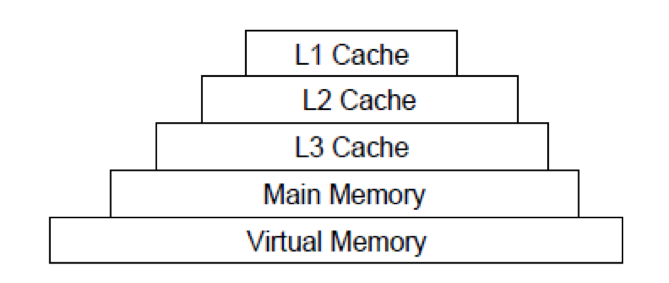
\includegraphics[width=\linewidth]{m5/memoryHierarchy}
\end{minipage}
\end{definition}

\begin{definition}{\textbf{Principles of Locality}}
	\begin{myitemize}
		\item \textbf{Spatial Locality}: If you've accessed a memory location, there's a very high chance that the next location you access is right next to it. E.g. executing instructions sequentially, accessing elements of an array.
		\item \textbf{Temporal Locality}: If you've accessed a memory location, there's a very high chance that you will access it again. E.g. Loops.
		\item \textbf{Note}: Because of locality, memory hierarchy allows you to have:
		\begin{myitemize}
			\item \textbf{Very fast memory}, since most accesses come from the fast top layer.
			\item \textbf{Very large memory}, since we can continue to keep what we don't (yet) need in the lowest layer.
		\end{myitemize}
	\end{myitemize}
\end{definition}

\begin{definition}{\textbf{Virtual Memory}}
	It is implemented on your hard disk! The layer above (your ``main memory'') maintains a copy of a small portion of the VM.
	
	We can do this by having instructions and data that the CPU is currently interested in, in main memory. Everything else stays on the VM. In this way we can squeeze MUCH MORE instructions and data than otherwise possible!
	
	\textbf{Paging}
	
	\begin{minipage}{0.5\linewidth}
		\begin{myitemize}
			\item VM is divided into fixed equal sized blocks called ``pages''. 
			\item Physical memory is divided into ``frames'' that are the same size as a VM page. A ``Virtual page'' in the VM can be loaded to any ``physical frame''  in main memory.
			\item The CPU always generates ``virtual addresses''. I.e. any CPU address always points to a page in virtual memory.
		\end{myitemize}
\end{minipage}
\begin{minipage}{0.25\linewidth}
	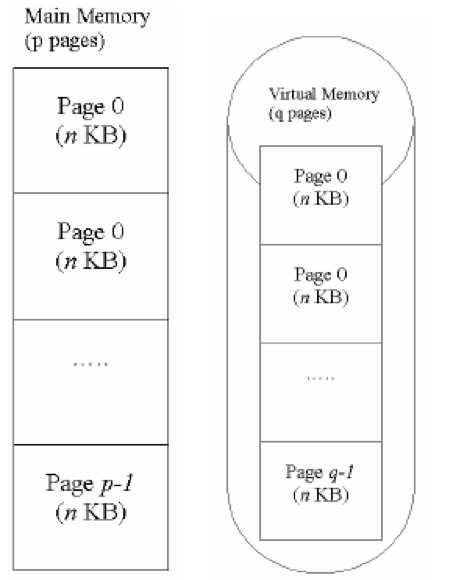
\includegraphics[width=1\linewidth]{m5/paging}
\end{minipage}
\begin{minipage}{0.25\linewidth}
	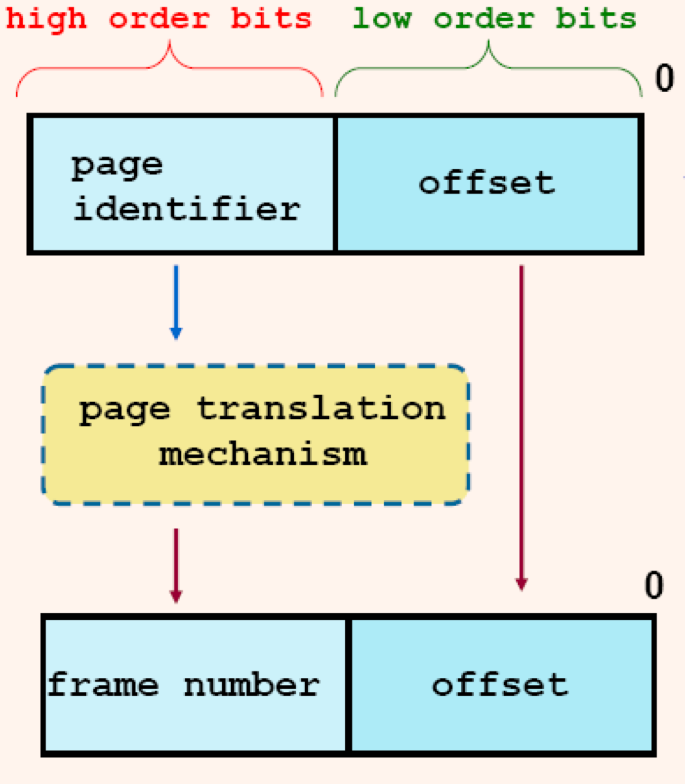
\includegraphics[width=1\linewidth]{m5/addressMapping}	
\end{minipage}

\textbf{Virtual to Physical Address Mapping}

\begin{minipage}{0.75\linewidth}
	\begin{myitemize}
		\item Virtual Page Number = Page Identifier; Frame number = Physical Page Number; Offset = Byte Index.
		\item Specialised hardware on the CPU, together with virtual memory services in the OS, work together to translate “virtual addresses” into “physical addresses” that correspond to locations in main memory.
		\item ``page table'': V=1 means the information requested is in main memory.
	\end{myitemize}
	
\end{minipage}
\begin{minipage}{0.25\linewidth}
	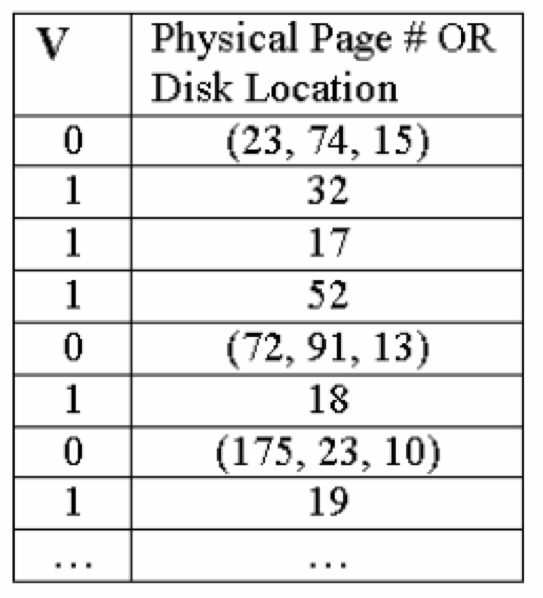
\includegraphics[width=.9\linewidth]{m5/pagetable}
\end{minipage}

\begin{minipage}{0.5\linewidth}
	\begin{myenumerate}
		\item The virtual address forms an index into the page table. If the ``virtual page'' is in memory, a ``memory translation'' process takes place that locates which frame this virtual page has been loaded into.
		\item This information is used to generate the ``physical address'' to access main memory.
	\end{myenumerate}
\end{minipage}
\begin{minipage}{0.5\linewidth}
	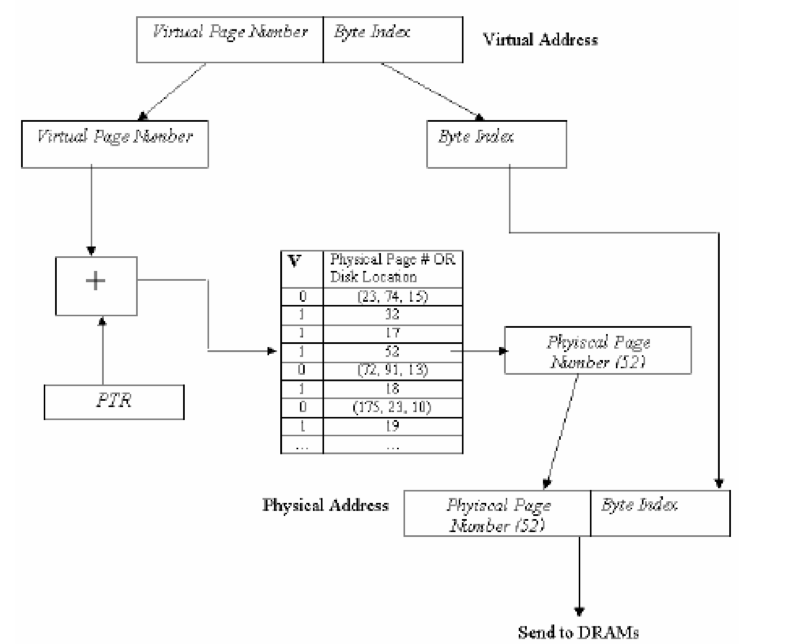
\includegraphics[width=.8\linewidth]{m5/translationProcedure}
\end{minipage}

\begin{myitemize}
	\item Given an N bit virtual addressing space, P bit physical addressing space with B byte page/frame size:
	\[\text{\# of bits in offset} = \log_2(B) \]
	\[\text{\# of bits in page identifier (or VPN)} = N - \log_2(B) \]
	\[\text{\# of bits in frame number} = P - \log_2(B) \]
	\item So if we have 32KB pages, a 4GB virtual addressing space and  2 GB of physical memory:
	\[\text{offset} =log2(32KB) = 15 \text{ bits}\]
	\[\text{Page identifier}: \log_2(4GB)-15=32-15=17 \text{ bits} \]
	\[\text{Frame number}: \log_2(2GB)-15=31-15=16 \text{ bits} \]
	There will be $2^{17}$ pages in this system, with $2^{16}$ frames.
	\item \textbf{Note}: 
	\begin{myenumerate}
		\item \textbf{No external fragmentation}: Pages that should be contiguous can be mapped to non-contiguous frames.
		\item \textbf{Internal fragmentation}: Basic allocation unit is now 1 page. Can be quite large!
		\item \textbf{Mapping is transparent} to programs. Programs only ``see'' virtual addresses.
		\item Can grow process segments by adding more pages. Growth is now limited to multiples of one page.
	\end{myenumerate}
	\item \textbf{Page Faults}: The V flag will be ``0''. The hardware sees this and generates a ``page fault'' interrupt. This is vectored to a “page fault” ISR within the OS.
	\begin{myenumerate}
		\item Locates where the missing page is on the disk: When V=0, the page table contains the location on disk where the page is (in cylinder/side/block format).
		\item Finds a free frame to load the VM page into.
		\item Updates the page table. Set V=1, and changes the entry to show which frame the virtual page has been loaded into.
		\item The VM then goes through the rest of the address translation process to allow the CPU to access the faulting data/instruction.
	\end{myenumerate}
	\item \textbf{Page loading policy}:
	\begin{myitemize}
		\item \textbf{Demand Paging}: Page is loaded when an access is made to a location inside it.
		\item \textbf{Pre-paging}: Other pages (e.g. surrounding pages) can be loaded together with the fault page. Pages can be pre-loaded when a process starts.
		\item Can be a mix of strategies.
	\end{myitemize}
	\item \textbf{Replacement policy}:
	\begin{myitemize}
		\item \textbf{FIFO}: 
		\begin{myitemize}
 			\item \textbf{Principle}: First page in = first page out.
		\item Use a FIFO queue of pages read in. New pages are added to the tail, pages at the head are swapped out when no more frames.
		\item \textbf{Belady's anomaly}: In a FIFO replacement policy, having more frames can increase paging instead of decreasing it.
		\item \textbf{Resolution}: consider frequency of use (i.e. temporal locality) instead of age. Optimal Page Replacement (OPT), Least Recently Used (LRU) and Clock Replacement (CR). None of these suffer from Belady's Anomaly.
		\end{myitemize}
		\item \textbf{LRU - Least Recently Used}
		\begin{myitemize}
			\item Each page table entry (PTE) has an p-bit counter $c_i$. At each access to page i, the $c_i$ is set to $2^p$. Counter for all other pages is decremented by 1.
			\item When it is time to replace a page: Perform a search through page table to find smallest $c_i$. Swap that page back to disk.
			\item If $>1$ page has smallest $c_i$, choose the first one we encountered.
		\end{myitemize}
		\end{myitemize}
		\item \textbf{Rewriting pages back to disk}: Pages are large. Writing swapped out pages back to disk is expensive. Have a ``D'' (Dirty) bit in each PTE. \textbf{Note}: requires hardware support to update D.
\end{myitemize}
\end{definition}

\begin{definition}{\textbf{Thrashing}}: a performance disaster
	When the amount of data/instructions in VM is much, much greater than available physical memory.
	\begin{myenumerate}
		\item Accessing instructions/data might frequently be in pages that aren't yet in physical memory.
		\item Shortage of physical memory causes frames to be frequently swapped out to disk.
		\item The swapped out frames are accessed again, causing other frames to be swapped out so that these can be swapped back in.
		\item Huge array, 4 million bytes. Random accesses will likely cause pages to be swapped out and back in again.
	\end{myenumerate}
\end{definition}

\begin{definition}{\textbf{Translation Lookaside}}

\begin{minipage}{0.5\linewidth}
	The page table is in main memory. \textbf{Two access}: One access to consult the page table. One access to actually read/write the physical memory. (Main memory is slower than the cache, therefore store parts of the page table in cache)
	\begin{myitemize}
		\item This special cache is called the ``Translation Lookaside Buffer'' or TLB. This is often located on the CPU die itself.

	\end{myitemize}
\end{minipage}\hspace{5mm}
\begin{minipage}{0.4\linewidth}
	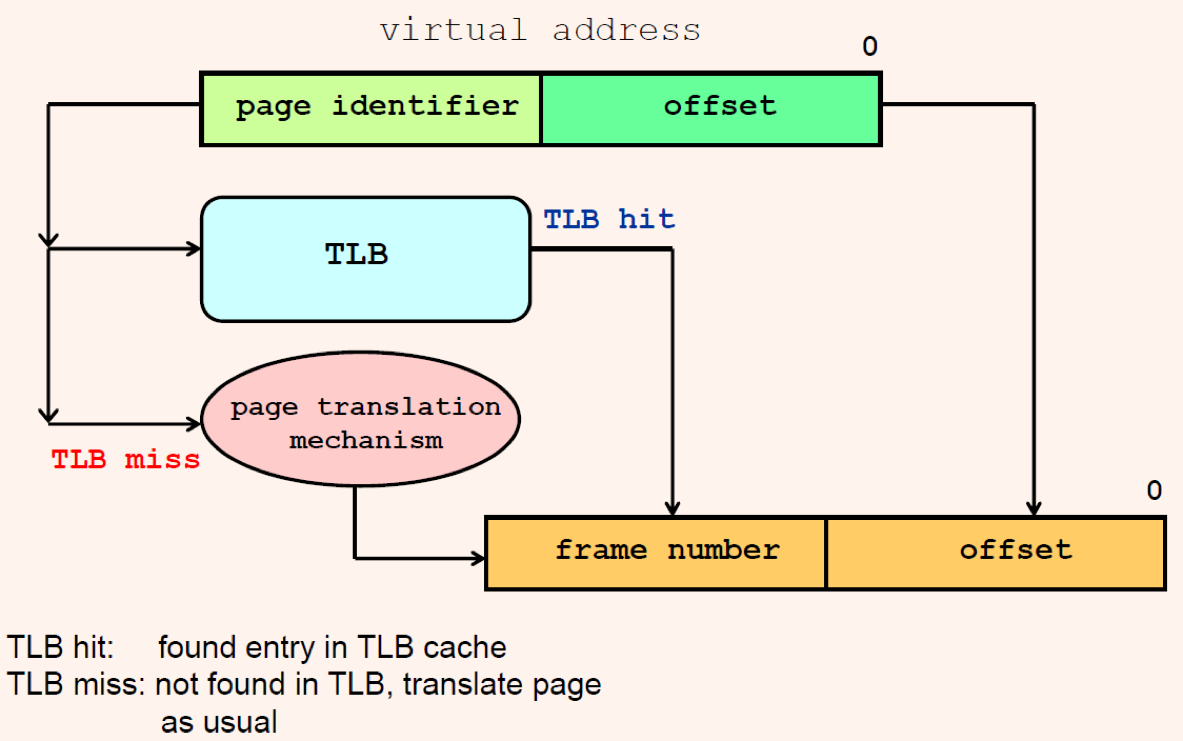
\includegraphics[width=\linewidth]{m5/translationLookasideBuffer}
\end{minipage}
	

\end{definition}









% $$$$$$$$$$$$$$$$$$$$$$$$$$$$$$$$$$ %
\end{document}